\documentclass[12pt,letterpaper]{article}
\usepackage{graphicx,textcomp}
\usepackage{natbib}
\usepackage{setspace}
\usepackage{fullpage}
\usepackage{color}
\usepackage[reqno]{amsmath}
\usepackage{amsthm}
\usepackage{fancyvrb}
\usepackage{amssymb,enumerate}
\usepackage[all]{xy}
\usepackage{endnotes}
\usepackage{lscape}
\newtheorem{com}{Comment}
\usepackage{float}
\usepackage{hyperref}
\newtheorem{lem} {Lemma}
\newtheorem{prop}{Proposition}
\newtheorem{thm}{Theorem}
\newtheorem{defn}{Definition}
\newtheorem{cor}{Corollary}
\newtheorem{obs}{Observation}
\usepackage[compact]{titlesec}
\usepackage{dcolumn}
\usepackage{tikz}
\usetikzlibrary{arrows}
\usepackage{multirow}
\usepackage{xcolor}
\newcolumntype{.}{D{.}{.}{-1}}
\newcolumntype{d}[1]{D{.}{.}{#1}}
\definecolor{light-gray}{gray}{0.65}
\usepackage{url}
\usepackage{listings}
\usepackage{color}

\definecolor{codegreen}{rgb}{0,0.6,0}
\definecolor{codegray}{rgb}{0.5,0.5,0.5}
\definecolor{codepurple}{rgb}{0.58,0,0.82}
\definecolor{backcolour}{rgb}{0.95,0.95,0.92}

\lstdefinestyle{mystyle}{
	backgroundcolor=\color{backcolour},   
	commentstyle=\color{codegreen},
	keywordstyle=\color{magenta},
	numberstyle=\tiny\color{codegray},
	stringstyle=\color{codepurple},
	basicstyle=\footnotesize,
	breakatwhitespace=false,         
	breaklines=true,                 
	captionpos=b,                    
	keepspaces=true,                 
	numbers=left,                    
	numbersep=5pt,                  
	showspaces=false,                
	showstringspaces=false,
	showtabs=false,                  
	tabsize=2
}
\lstset{style=mystyle}
\newcommand{\Sref}[1]{Section~\ref{#1}}
\newtheorem{hyp}{Hypothesis}

% highlighting tools to identify final answer
\definecolor{pastelyellow}{RGB}{255, 250, 205}
\usepackage{soul}
\sethlcolor{pastelyellow}

\title{Problem Set 2}
\date{Due: October 22, 2026}
\author{Emily Zhang}

\begin{document}
	\maketitle
	\section*{Instructions}
\begin{itemize}
	\item Please show your work! You may lose points by simply writing in the answer. If the problem requires you to execute commands in \texttt{R}, please include the code you used to get your answers. Please also include the \texttt{.R} file that contains your code. If you are not sure if work needs to be shown for a particular problem, please ask.
	\item Your homework should be submitted electronically on GitHub.
	\item This problem set is due before 23:59 on Thursday October 22, 2026. No late assignments will be accepted.

\end{itemize}

	
	\vspace{.5cm}
	\section*{Question 1: Political Science}
		\vspace{.25cm}
	The following table was created using the data from a study run in a major Latin American city.\footnote{Fried, Lagunes, and Venkataramani (2010). ``Corruption and Inequality at the Crossroad: A Multimethod Study of Bribery and Discrimination in Latin America. \textit{Latin American Research Review}. 45 (1): 76-97.} As part of the experimental treatment in the study, one employee of the research team was chosen to make illegal left turns across traffic to draw the attention of the police officers on shift. Two employee drivers were upper class, two were lower class drivers, and the identity of the driver was randomly assigned per encounter. The researchers were interested in whether officers were more or less likely to solicit a bribe from drivers depending on their class (officers use phrases like, ``We can solve this the easy way'' to draw a bribe). The table below shows the resulting data.


\begin{table}[h!]
	\centering
	\begin{tabular}{l | c c c }
		& Not Stopped & Bribe requested & Stopped/given warning \\
		\\[-1.8ex] 
		\hline \\[-1.8ex]
		Upper class & 14 & 6 & 7 \\
		Lower class & 7 & 7 & 1 \\
		\hline
	\end{tabular}
\end{table}

	\textit{Set Up the Data Table (with Row and Column Totals):}
	\lstinputlisting[language=R, firstline=39, lastline=58]{PS02_answersEZ.R}

\begin{enumerate}
	
	\item [(a)]
	Calculate the $\chi^2$ test statistic by hand/manually (even better if you can do "by hand" in \texttt{R}).\\
	
	\textit{Null and Alternate Hypotheses:}
	
	\[
	\begin{aligned}
		H_0 &: \text{Social class and police extortion are statistically independent} \\
		H_A &: \text{Social class and police extortion are statistically dependent}
	\end{aligned}
	\]
	
	\textit{Expected Frequencies:}
	\lstinputlisting[language=R, firstline=75, lastline=97]{PS02_answersEZ.R}
	
	\textit{Chi-Square Test Statistic:}
	\lstinputlisting[language=R, firstline=105, lastline=125]{PS02_answersEZ.R}
	
	\textit{Check Using the Built-in \texttt{chisq.test()} Function:}
	\lstinputlisting[language=R, firstline=127, lastline=127]{PS02_answersEZ.R}
	
	\textbf{Analysis:}\\
	To calculate the $\chi^2$ test statistic, we first need the expected frequency of each cell under the null hypothesis of independence. Each expected frequency is calculated by multiplying the row total by the column total and dividing by the grand total of 42 observations. For example, the expected number of upper class drivers who were not stopped is $\frac{27 \times 21}{42} = 13.5$. I wrote a small function for this calculation and applied it to every cell using a nested for loop, which gives the expected frequencies in the table below.
	
	\begin{table}[H]
		\centering
		\caption{\footnotesize Expected Frequencies}
		\begin{tabular}{l | c c c }
			& Not Stopped & Bribe requested & Stopped/given warning \\
			\\[-1.8ex] 
			\hline \\[-1.8ex]
			Upper class & 13.500 & 8.357 & 5.143 \\
			Lower class & 7.500 & 4.643 & 2.857 \\
			\hline
		\end{tabular}
	\end{table}
	
	With the expected frequencies, I then wrote a second function that loops through each of the six cells and adds up the squared difference between the observed and expected frequency, divided by the expected frequency, which follows the formula $\chi^2 = \sum \frac{(f_o - f_e)^2}{f_e}$. This result was verified against the built-in \texttt{chisq.test()} function, which gives the same value.
	
	\hl{The {$\chi^2$} test statistic is 3.791.}
	
	\vspace{.5cm}
	
	\item [(b)]
	Now calculate the p-value from the test statistic you just created (in \texttt{R}).\footnote{Remember frequency should be $>$ 5 for all cells, but let's calculate the p-value here anyway.}  What do you conclude if $\alpha = 0.1$?\\
	
	\textit{Checking the Assumption (Expected Frequencies $\geq 5$):}
	\lstinputlisting[language=R, firstline=131, lastline=154]{PS02_answersEZ.R}
	
	\textit{Degrees of Freedom and P-value:}
	\lstinputlisting[language=R, firstline=156, lastline=160]{PS02_answersEZ.R}
	
	\textbf{Analysis:}\\
	Before calculating the p-value, I first checked the assumption that all expected frequencies are at least 5. Using a for loop, I counted the cells that violate this assumption. Two of the six cells, namely lower class drivers who were asked for a bribe (4.643) and lower class drivers who were stopped or given a warning (2.857), have expected frequencies below 5, so the assumption is not met. Hence, the result should be interpreted cautiously.
	
	The degrees of freedom for a chi-square test of independence is $(r-1)(c-1)$, where $r$ is the number of rows and $c$ is the number of columns. With two rows and three columns, we have $(2-1)(3-1) = 2$ degrees of freedom. Then, I used the built-in \texttt{pchisq()} function with \texttt{lower.tail = FALSE} to obtain the area in the right tail of the distribution, since the chi-square test is always a one-tailed test, which gives a p-value of 0.150.
	
	Using the significance level of $\alpha = 0.1$, we observe that the p-value of 0.150 is greater than $\alpha$. This indicates that in a world where the null hypothesis is true, it is not unlikely to observe a test statistic as extreme as 3.791. With that in mind, we would fail to reject the null hypothesis.
	
	\hl{We fail to reject the null hypothesis and can conclude that there is not sufficient evidence to say that social class and police extortion are statistically dependent. However, because two expected counts were below 5, the assumption was not met and the result should be interpreted cautiously.}
	
	\vspace{.5cm}
	
	\item [(c)] Calculate the standardized residuals for each cell and put them in the table below.
	
	\textit{Standardised Residuals:}
	\lstinputlisting[language=R, firstline=170, lastline=196]{PS02_answersEZ.R}
	
	\begin{table}[H]
		\centering
		\caption{\footnotesize Standardised Residuals}
		\begin{tabular}{l | c c c }
			& Not Stopped & Bribe requested & Stopped/given warning \\
			\\[-1.8ex] 
			\hline \\[-1.8ex]
			Upper class  & 0.322 & $-1.642$ & 1.523 \\
			\\
			Lower class & $-0.322$ & 1.642 & $-1.523$ \\
			\hline
		\end{tabular}
	\end{table}
	
	\textbf{Analysis:}\\
	The standardised residual of each cell is calculated with the formula
	\[
	\frac{f_o - f_e}{\sqrt{f_e\left(1-\frac{\text{row total}}{\text{grand total}}\right)\left(1-\frac{\text{column total}}{\text{grand total}}\right)}}.
	\]
	In other words, the observed minus the expected frequency is divided by an estimate of its standard error. Similar to the previous parts, I wrote a function for this formula and applied it to each cell with a nested for loop. Because the table only has two rows, the residuals of the upper class and lower class are equal in magnitude but opposite in sign.
	
	\vspace{.5cm}
	
	
	\item [(d)] How might the standardized residuals help you interpret the results?  
	
	textbf{Analysis:}\\
	The standardised residuals measure the strength of the difference between the observed and expected frequencies within each cell. Because they are standardised, we can base our interpretation on the normal distribution. According to the empirical rule, approximately 95\% of the data should fall between -2 and +2 standard deviations of the mean, so any standardised residual outside of these bounds indicates a cell that departs notably from independence. 
	
	Using the cutoff of $|z| > 2$, no cell shows a significant departure from independence, which is consistent with the non-significant chi-square test in part (b). The cells with the highest standardised residuals are the ``Bribe requested'' and ``Stopped/given warning'' categories at $|1.642|$ and $|1.523|$ respectively, in comparison to the ``Not Stopped'' category at $|0.322|$. This pattern weakly suggests that upper class drivers were asked for bribes less often than expected, while upper class drivers were stopped and given a warning more often than expected. The opposite is true for lower class drivers. However, none of these deviations is large enough to conclude that social class and police extortion are dependent, and the small expected counts mean that this pattern should be interpreted cautiously.
	
	\hl{The standardised residuals show that no single cell drives the result, which is consistent with failing to reject the null hypothesis that social class and police extortion are independent.}
	
\end{enumerate}

\newpage
	
\section*{Question 2: Economics}
Chattopadhyay and Duflo were interested in whether women promote different policies than men.\footnote{Chattopadhyay and Duflo. (2004). ``Women as Policy Makers: Evidence from a Randomized Policy Experiment in India. \textit{Econometrica}. 72 (5), 1409-1443.} Answering this question with observational data is pretty difficult due to potential confounding problems (e.g. the districts that choose female politicians are likely to systematically differ in other aspects too). Hence, they exploit a randomized policy experiment in India, where since the mid-1990s, $\frac{1}{3}$ of village council heads have been randomly reserved for women. A subset of the data from West Bengal can be found at the following link: \url{https://raw.githubusercontent.com/kosukeimai/qss/master/PREDICTION/women.csv}\\

\noindent Each observation in the data set represents a village and there are two villages associated with one GP (i.e. a level of government is called "GP"). Figure~\ref{fig:women_desc} below shows the names and descriptions of the variables in the dataset. The authors hypothesize that female politicians are more likely to support policies female voters want. Researchers found that more women complain about the quality of drinking water than men. You need to estimate the effect of the reservation policy on the number of new or repaired drinking water facilities in the villages.
\vspace{.5cm}
\begin{figure}[h!]
	\caption{\footnotesize{Names and description of variables from Chattopadhyay and Duflo (2004).}}
	\vspace{.5cm}
	\centering
	\label{fig:women_desc}
	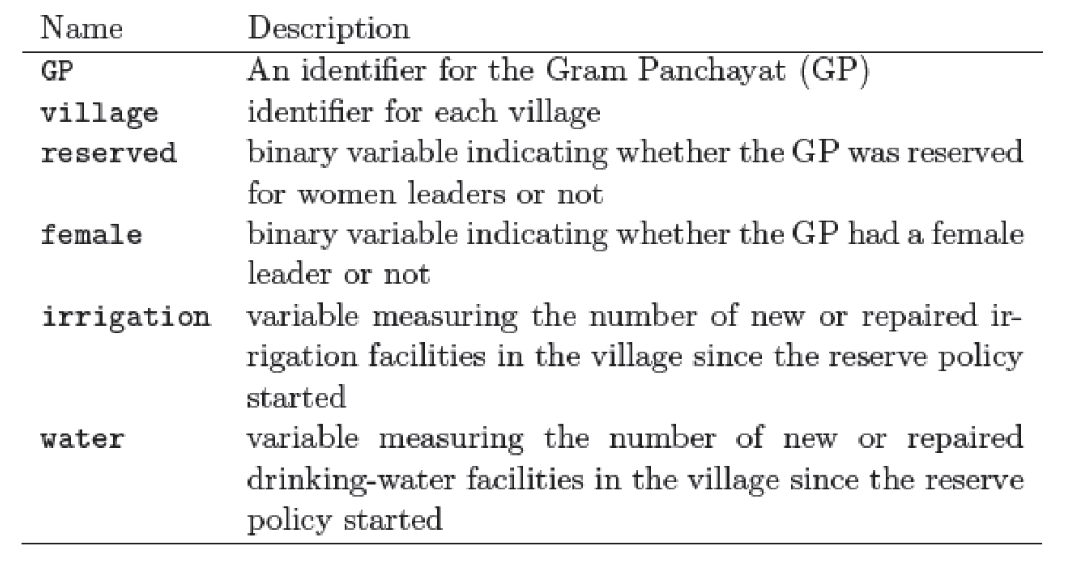
\includegraphics[width=\textwidth]{women_desc.png}
\end{figure}		

\textit{Import and Explore Data:}
\lstinputlisting[language=R, firstline=219, lastline=223]{PS02_answersEZ.R}

\begin{enumerate}
	\item [(a)] State a null and alternative (two-tailed) hypothesis. 
	
	\item [(a)] State a null and alternative (two-tailed) hypothesis. \\
	
	\[
	\begin{aligned}
		H_0 &: \beta_1 = 0 &\qquad \text{(no effect of the reservation policy)} \\
		H_A &: \beta_1 \neq 0 &\qquad \text{(an effect of the reservation policy)}
	\end{aligned}
	\]
	
	\textbf{Analysis:}\\
	The outcome variable is \texttt{water}, the number of new or repaired drinking water facilities in a village, and the explanatory variable is \texttt{reserved}, a binary variable indicating whether the GP was reserved for women leaders. Because the question asks for a two-tailed test, the alternative hypothesis does not specify a direction. The null hypothesis states that there is no linear relationship between the reservation policy and the number of new or repaired drinking water facilities in the villages, such that the slope coefficient $\beta_1$ is zero. In contrast, the alternative hypothesis states that there is a linear relationship, such that $\beta_1$ is not zero.
	
	\vspace{.5cm}
	
	\item [(b)] Run a bivariate regression to test this hypothesis in \texttt{R} (include your code!).
	
	\textit{Slope Estimate:}
	\lstinputlisting[language=R, firstline=232, lastline=250]{PS02_answersEZ.R}
	
	\textit{Intercept, Standard Error, T-statistic, and P-value:}
	\lstinputlisting[language=R, firstline=252, lastline=263]{PS02_answersEZ.R}
	
	\textit{Check Using the Built-in \texttt{lm()} Function:}
	\lstinputlisting[language=R, firstline=265, lastline=266]{PS02_answersEZ.R}
	
	\begin{table}[H]
		\centering
		\caption{\footnotesize Bivariate Regression of Water Facilities on Reservation Policy}
		\begin{tabular}{l | c c c c}
			& Estimate & Std. Error & t value & $\Pr(>|t|)$ \\
			\\[-1.8ex] 
			\hline \\[-1.8ex]
			Intercept & 14.738 & 2.286 & 6.446 & $<0.001$ \\
			Reserved & 9.252 & 3.948 & 2.344 & 0.0197 \\
			\hline
			\multicolumn{5}{l}{\footnotesize $n = 322$, \; Residual standard error = 33.45 on 320 df, \; $R^2 = 0.017$}
		\end{tabular}
	\end{table}
	
	\textbf{Analysis:}\\
	Rather than relying only on the built-in function, I first calculated the regression by hand. The slope estimate is $\hat{\beta}_1 = \frac{\sum (x_i - \bar{x})(y_i - \bar{y})}{\sum (x_i - \bar{x})^2}$, which I calculated with a for loop, and the intercept is $\hat{\beta}_0 = \bar{y} - \hat{\beta}_1 \bar{x}$. Then, I used the fitted values to calculate the sum of squared errors, which gives the residual standard error with $n-2$ degrees of freedom. Dividing this by $\sqrt{\sum (x_i - \bar{x})^2}$ gives the standard error of the slope, and dividing the slope by its standard error gives the t-statistic of 2.344. The two-tailed p-value is obtained with \texttt{pt()}, using the absolute value of the t-statistic and $n-2 = 320$ degrees of freedom, and multiplying it by two to account for both tails, which gives 0.0197. All of these values are identical to the output of the built-in \texttt{lm()} function.
	
	
	\vspace{.5cm}
	
	\item [(c)] Interpret the coefficient estimate for reservation policy. 
	
	\textit{Significance Level:}
	\lstinputlisting[language=R, firstline=270, lastline=271]{PS02_answersEZ.R}
	
	\textbf{Analysis:}\\
	The coefficient estimate for the reservation policy is 9.252. Since \texttt{reserved} is a binary variable, the coefficient is the difference in the average number of new or repaired drinking water facilities between villages in reserved GPs and villages in non-reserved GPs. In other words, on average, villages in GPs that are reserved for women have approximately 9.25 more new or repaired drinking water facilities than villages in GPs that are not reserved. This is also supported by the group means, since the intercept of 14.738 is the average number of facilities in non-reserved villages, and the average in reserved villages is $14.738 + 9.252 = 23.991$.
	
	With a significance level of $\alpha = 0.05$, we observe that the p-value of 0.0197 is less than $\alpha$. Hence, we have sufficient evidence to reject the null hypothesis and can say that there is a linear relationship between the reservation policy and the number of new or repaired drinking water facilities in the villages. Because the reservation policy was randomly assigned, we can also interpret this relationship as causal. However, it is important to note that the p-value of 0.0197 is not statistically significant if the alpha threshold is changed to 0.01. By assuming a threshold of 0.05, I am accepting a 5\% risk of a false positive, that is rejecting a true null hypothesis. Furthermore, the $R^2$ of 0.017 indicates that the reservation policy explains only a small share of the variation in the number of water facilities across villages, so the policy is only one of many factors that matter.
	
	We also observe from our linear regression model that the intercept has a p-value almost at 0, which is less than the alpha level of 0.05. This indicates that the average number of water facilities in non-reserved villages is significantly different from 0. From a real-world standpoint, this is not necessarily abnormal because the non-reserved villages probably do get some new or repaired water facilities, so it would be unlikely to assume that the control group should average exactly zero facilities.
	
	\hl{On average, villages in GPs reserved for women have 9.252 more new or repaired drinking water facilities than villages in non-reserved GPs, and this difference is statistically significant at the 0.05 level (p = 0.0197) but not at the 0.01 level.}
	
\end{enumerate}


%\end{enumerate}
\end{document}
